\documentclass{article}
\usepackage[utf8]{inputenc}
\usepackage[margin= 1in]{geometry}
\usepackage[utf8]{inputenc}
\usepackage[none]{hyphenat}
\usepackage{parskip}
\usepackage{multicol}
\usepackage{listings}  
\usepackage[numbered,framed]{matlab-prettifier}
\usepackage[T1]{fontenc}
% standard packages
\usepackage{subcaption}
\usepackage{enumerate}
\usepackage{nccmath}
\usepackage{svg}
\usepackage{mathtools}
\usepackage{float}
\usepackage{scrextend}
\usepackage{fancyhdr}
\usepackage{fancyvrb}
%\usepackage{bickham}
% \usepackage{BOONDOX-cal[o]}
%\usepackage{boondox-calo}
\usepackage{dutchcal}
\usepackage{minted}
\usepackage{hyperref}
% math packages
\usepackage{centernot}
\usepackage{amsthm, amssymb, amsmath,verbatim}
\usepackage{mathtools}
% coding and colors
\usepackage{xifthen}
\usepackage{xcolor}
\usemintedstyle{borland}
\usepackage{ifthen}

% color box
\usepackage[most,listings]{tcolorbox}
\usepackage{lmodern}
% graphs and pictures
\usepackage{mathrsfs}
\usetikzlibrary{math}
\usetikzlibrary{backgrounds}
\usetikzlibrary{patterns,calc}
\usepackage{graphicx, subcaption}
\usepackage{csvsimple,booktabs}
\usepackage{filecontents}
\theoremstyle{definition}
\newtheorem{definition}{Definition}[section]
\newtheorem{theorem}{Theorem}[section]
\newtheorem{assmp}{Assumption}[section]
\usepackage{geometry}
\geometry{
	%margin = 14.11mm, tmargin = 0.4 in
	margin = 15mm, bmargin = 0.in, tmargin = 0.4in
}

%\usepackage{bbm}
\usepackage{authblk}

\usepackage{mathtools}

\newcommand{\R}{\mathcal{R}}
\newcommand{\SA}{\mathcal{S}}
\newcommand{\E}{\mathcal{E}}
\newcommand{\F}{\mathcal{F}}
\newcommand{\U}{\mathcal{U}}

\usepackage[ruled,vlined]{algorithm2e}
\def\course{Course \#: Course Title}      %Course
\def\thetitle{Report Title}               % Report Title
\def\Headauthor{last name et al.}         % Header Authors of work
\def\date{\today}                         % Date
\usepackage{array}
\newcommand{\PreserveBackslash}[1]{\let\temp=\\#1\let\\=\temp}
\newcolumntype{C}[1]{>{\PreserveBackslash\centering}p{#1}}
\newcolumntype{R}[1]{>{\PreserveBackslash\raggedleft}p{#1}}
\newcolumntype{L}[1]{>{\PreserveBackslash\raggedright}p{#1}}
\begin{document}

\begin{center}
    \vspace*{1.5cm}
    % University Logo
    
\includegraphics[scale = 0.5]{iitb-logo.png}\\[1.75cm]
    % University Name
    \textsc{\color[RGB]{0, 51, 102}\LARGE{Indian Institute of Technology Bombay}}\\[1cm]
    \textsc{\Large{EE 691 RnD Project}}\\[.5cm]
    \textsc{\Large{Average Reward Deep Reinforcement Learning}}\\[.5cm]
    \textsc{\date}\\[2cm]
    \Large{
    \begin{tabular}{L{4cm} R{4cm}}
        \textit{Author} &  \textit{Roll Number}\\
        \hline
        % author names and PID
        Tejas Pagare & 190070067
    \end{tabular}
    }\\
    \vspace{1cm}
    \textit{under the guidance of}
    \\\vspace{1cm}
    Prof. Vivek Borkar\\
    \vspace{0.2cm}
    \textit{Electrical Engineering, IIT Bombay}\\[.5cm]
    
\end{center}
\thispagestyle{empty}
\pagebreak

\newgeometry{
	a4paper,margin = 15mm,top=25mm,bottom=25mm,bindingoffset=6mm
}
\clearpage
\vspace*{\fill}
\begin{center}
    % \begin{minipage}{25em}
    \begin{center}
        \Large{$\mathcal{{dedicated\ to\ Aai}}$}
    \end{center}
    
    % \vspace{10pt}
    % \textit{We propose Average reward DQN algorithm and state it's applications in several domains including restless bandits.} 
    % \end{minipage}
\end{center}
\vspace*{\fill}
\clearpage
\pagestyle{fancy}
\tableofcontents
\clearpage

\section{Preliminaries}
\subsection{Finite-State Markov Chains}
\begin{definition}[]A Finite Markov chain is an integer-time process i.e. \{$X_n, n\geq0$\} where each $X_n$ is a random variable from a countable finite set $\mathcal{S}$ and we have
\[\text{Pr}\{X_n=j|X_{n-1}=i,X_{n-2}=k,\dotsc,X_0=m\} = \text{Pr}\{X_n=j|X_{n-1}=i\} = P_{ij}\]
which says that state $X_n$ is independent of past states given the last state $X_{n-1}$ and further it doesn't depend on $n$. 
We denote the pair \{$\mathcal{S},\mathcal{P}$\} as a stationary finite-state markov chain, where $\mathcal{S}$ is finite set of states and $\mathcal{P}$ is a stochastic matrix or state transition probability matrix with $P_{ij}$ as its elements.
\end{definition}

\subsubsection*{Classification of states of a finite-state markov chain \{$\mathcal{S},\mathcal{P}$\}}

Denoting \text{Pr}\{$X_n=j|X_0=i$\} = $P_{ij}^{n}$ as Probability that after $n^{th}$ transition $X_n=j$ starting from initial state $X_0=i$.

A state $j$ is accessible from state $i$ ($i\rightarrow j$) iff \text{Pr}\{$X_n=j|X_0=i$\} > 0 for some $n\geq1$.

Two state $i$ and $j$  communicate ($i\leftrightarrow j$) if i is accessible from j and j is accessible from i (i.e. $i\rightarrow j$ and $j\rightarrow i$) or if there exists two positive integers $k_1$ and $k_2$ such that $P_{ij}^{k_1}$ > 0 and $P_{ji}^{k_1}$ > 0. 
\begin{definition}[] For finite-state Markov chains, a recurrent state is a state $i$ that is
accessible from all states that are accessible from $i$ ($i$ is recurrent if $i\rightarrow j$ implies that
$j\rightarrow i$). A transient state is a state that is not recurrent. A state $i$ is transient if there is some $j$ that is accessible from $i$ but from which there is no possible return.
\end{definition}

\begin{definition}
A class $\mathcal{C}$ of states is a non-empty set of states such that each $i \in \mathcal{C}$
communicates with every other state $j \in \mathcal{C}$ and communicates with no $j \not\in \mathcal{C}$.
\end{definition}
A recurrent or ergodic class therefore is a set of recurrent states that all communicate with each other and do not communicate with states outside this class.
\begin{theorem}
For finite-state Markov chains, either all states in a class are transient or all are recurrent.

If $\mathcal{S}$ itself is a recurrent class then we say that the Markov chain is \textbf{irreducible}. 

We have $\underset{k\rightarrow\infty}{\text{lim}} P_{ij}^k=0$ iff i is transient.

\textbf{Main takeaway} - If the process starts in a recurrent class, it stays within that class. If it starts in a recurrent class, it eventually enters in a recurrent class (with probability one) after a finite number of transitions, and hence subsequently remains there.\\
Please refer to \cite{markovmit} and Appendix D of \cite{dp1} for detailed description.
\end{theorem}


\subsection{Markov Decision Processes}
\begin{definition}
A MDP consists of 
\begin{itemize}
    \item A set of states $\mathcal{S}$, set of actions $\mathcal{A}$ for moving from a state to another. $\mathcal{S}$ and $\mathcal{A}$ can be both finite or infinite.
    \item Transition Probabilities $P$ which is defined the probability distribution over next states given the current state and current action where $P_{ij}(a) = \text{Pr}\{X_{n+1}=j|X_{n}=i,U_n=a\}$.
    \item A reward function which is defined as $\mathcal{R}: \mathcal{S}\times\mathcal{A}\rightarrow\mathbb{R}$, where $\mathcal{R}_s^a$ or $r(s,a)$ is the expected reward of taking action $a$ in state $s$.
\end{itemize} 

Therefore a MDP is simply given as a pair $(\mathcal{S},\mathcal{A},\mathcal{R})$.\\
\end{definition}
A policy $\pi:\mathcal{S}\rightarrow\mathcal{A}$ is a distribution over actions given states $\pi(a|s) = \text{Pr}\{U_n=a|X_n=s\}$. \\For stationary policy we have $U_n\sim \text{Pr}(\cdot|X_n=s)$ $\forall t>0$.\clearpage
Any policy induces a Markov chain whose transition probability or stochastic matrix is denoted as $P(\pi) \in [0,1]^{|\mathcal{S}|\times|\mathcal{S}|}$  where each entry $P_{ij}(\pi) = \sum_{a\in\mathcal{A}}\pi(a|s)p(j|i,a)$. This Markov chain is denoted as $(\mathcal{S},\mathcal{P}(\pi))$.\\

Below definitions for MDPs are simply the extensions of the Markov chains under a stationary policy. \\
We say that a state $i$ is accessible from state $j$ if there exists a stationary policy $\pi$ and an integer k such that $P(x_k=j|x_0=i,\pi)>0$
\begin{definition}
An MDP is ergodic or recurrent if the Markov chain induced by any stationary policy is ergodic or the transition matrix of the induced Markov chain has a single recurrent class.
\end{definition}
\begin{definition}
\label{def:unichain}
An MDP is unichain if it consists of a single recurrent class and possibly some transient states.
\end{definition}
An MDP is communicating if every pair of states communicate with each other under a stationary policy.
\begin{definition}
MDPs in which at least one policy results in two or more closed communicating classes (recurrent classes) and a transient class (possibly empty) are called Multichain
MDPs.
\end{definition}

A broader condition known as \textit{Weak Accessibility} from Chapter 4. of \cite{dp1} is important for most of the results to hold.
\begin{definition}
A Weak Accessibility (WA) condition holds if the set of states can be partitioned into two subsets $S_t$ and $S_c$ such that:\\
(i) All states in $S_t$ are transient under every stationary policy.\\
(ii) For every two states $i$ and $j$ in $S_c$, $j$ is accessible from $i$.
\end{definition}

% Refer to \cite{mdpsilver} for broader understanding of MDPs.

\subsection{Average Reward Problems}
Please refer to \cite{dp2,survey,Mahadevan2005AverageRR} for a broader view.\\
The objective here is to maximize over all policies $\pi=\{\mu_0,\mu_1,\dotsc\}$ where $\mu_n(i)\in U(i)$ denotes the \textit{valid action in state i} for all $i$ and $n$, the expected average reward per stage (also termed as gain) starting from a state $i$.
\begin{equation}
    \label{eqn:def}
    \rho^{\pi}(i)=\underset{N\rightarrow\infty}{\text{lim inf}}\dfrac{1}{N}E\Big\{\sum_{n=0}^{N-1}r(x_n,\mu_n(x_n))|x_0=i\Big\}
\end{equation}
where $r$ denotes the instantaneous reward incurred after taking action $\mu_n(x_n)$ in state $x_n$. Here, lim inf is used as opposed to lim to justify the fact that lim may not generally exist.\\
% When the limit in Eq. (\ref{eqn:def}) doesn't exists we define upper and lower rewards of a policy as 
% \begin{align*}
%     \rho_{\pi}^{+}(i)&=\underset{N\rightarrow\infty}{\text{lim sup}}\dfrac{1}{N}E\Big\{\sum_{k=0}^{N-1}r(x_n,\mu_n(x_n))|x_0=i\Big\}\\
%     \rho_{\pi}^{-}(i)&=\underset{N\rightarrow\infty}{\text{lim inf}}\dfrac{1}{N}E\Big\{\sum_{k=0}^{N-1}r(x_n,\mu_n(x_n))|x_0=i\Big\}
% \end{align*}
% and for the policies $\pi$ of interest we have $\rho_{\pi}^{+}(i)=\rho_{\pi}^{-}(i)$ and this value is referred to as reward incurred (or gain) by $\pi$ starting from state $i$.\\

We note that, rewards incurred in the early stage do not matter since their contribution to the average reward per stage is reduced to zero as $N\rightarrow\infty$
\begin{equation}
    \label{eqn:finite}
    \underset{N\rightarrow\infty}{\text{lim}}\dfrac{1}{N}E\Big\{\sum_{n=0}^{K}r(x_n,\mu_n(x_n))|x_0=i\Big\}=0
\end{equation}
for any fixed $K$.\\
\[\therefore \rho^\pi(i)=\rho^\pi(j)\ \forall i,j\ \text{with} \ E\{N_{ij}(\pi)\}<\infty\] \\
where $N_{ij}(\pi)$ denotes the time of first visit to state $j$ starting from state $i$ and this condition is equivalent to saying that the system reaches $j$ starting from $i$ with probability 1.\\

\begin{definition}
A gain optimal policy $\pi*$ is defined as the policy which maximizes the average reward for all states i.e.
\begin{center}
    $\pi^*$ is gain optimal if $\rho^{\pi^*}(s_0)\geq\rho^{\pi}(s_0)$ $\forall \pi$ and $\forall s_0 \in \mathcal{S}$\\
and hence $\pi^* \in \underset{\pi}{\text{arg max}} \rho^\pi$
\end{center}

Now, we refer to the general case of unichain MDPs which follows the broader \textit{Weak Accessibility} criteria and hence shown the existence of Blackwell optimality policies refer Definition \ref{def:blackwell}.
We now state the important result that for unichain MDPs, the average reward for any stationary policy is independent of the initial state. 
\begin{center}
    $\rho^{\pi}(s) = \rho^{\pi}(s') = \rho^\pi$ $\forall \pi$ and $\forall s,s' \in \mathcal{S}$
\end{center}
    

This can be shown by a simple lookup of the unichain condition Definition \ref{def:unichain}. 
\\Since, we know that the states in the recurrent class will be visited forever and hence the expected average reward cannot differ across the states in the recurrent class. \\Now, for transient states we know that they will be never be reentered after we are in recurrent class, hence the transient states accumulate a finite total expected reward. This finite reward vanishes under the limit as stated in Eq. (\ref{eqn:finite})
\end{definition}

We define bias value  $V_b^\pi(s_0)$ as the average adjusted sum of rewards from a policy
\begin{equation}
    V_b^\pi(s_0) := \underset{N\rightarrow\infty}{\text{lim}} E\Big\{\sum_{n=0}^{N-1}\Big(r(x_n,\mu_n(x_n))-\rho^\pi\Big)|x_0=s_0\Big\}
\end{equation}
where $\rho^\pi$ is the average reward associated with the policy $\pi$.\\
This bias value or relative value has the interpretation of relative difference in total reward gained by starting from some state $s$ as opposed to starting from some other state $s'$ which can be shown by following:
\[\because V_b^\pi(s)-V_b^\pi(s') = \underset{N\rightarrow\infty}{\text{lim}}\Bigg[E\Big\{\sum_{n=0}^{N-1}r(x_n,\mu_n(x_n))|x_0=s\Big\} -  E\Big\{\sum_{n=0}^{N-1}r(x_n,\mu_n(x_n))|x_0=s'\Big\}\Bigg]\]\\

\begin{definition}
A policy $\pi^*$ is termed as \textit{bias optimal} if it is gain optimal and it maximizes the bias values i.e. $V_b^{\pi^*}(s)\geq V_b^{\pi}(s) \forall s \in \mathcal{S}$ and stationary policies $\pi$.
\end{definition}

\begin{definition}
\label{def:blackwell}
A stationary policy $\pi$ is said to be \textit{Blackwell optimal} if it is simultaneously optimal for all the $\alpha$-discounted problems with $\alpha$ in an interval $(\overline{\alpha},1)$ where $\overline{\alpha}$ is some scalar with $0<\overline{\alpha}<1$.
\end{definition}



\subsubsection{Bellman Equation}
\begin{theorem}
For any unichain MDP, there exists a value function $V^*$ and a scalar $\rho^*$ satisfying the equation.
\begin{equation}
    \label{eqn:bellman}
    V^*(s)+\rho^* = \underset{a}{\text{max}}\Big\{r(s,a)+ \sum_{s'\in\mathcal{S}}p(s'|s,a)V^*(s')\Big\}  \hspace{10pt} \forall s \in \mathcal{S}
\end{equation}
The greedy policy $\pi^*$ which selects action by maximizing the RHS of this equation achieves optimal average reward $\rho^* = \rho^{\pi^*}$ and is a gain-optimal policy.
\end{theorem}
\section{Value Iteration Methods}
We consider a controlled Markov chain $\{X_n\}$ on a finite state space $\mathcal{S} = \{1,2,\dotsc,d\}$  with a finite action space $\mathcal{A} = \{a_1,\dotsc,a_r\}$ and transition probabilities $p(\cdot|s,a)$.\\
\textbf{Also, from now on we assume Unichain condition (Definition \ref{def:unichain}) throughout unless specified.}\\

Consider the mapping $T(V)(s)$ obtained by applying RHS of the Bellman equation (\ref{eqn:bellman})
\begin{equation}
    T(V)(s) = \underset{a}{\text{max}} \Big(r(s,a)+\sum_{s'}p(s'|s,a)V(s') \Big)
\end{equation}
This mapping is shown to be a monotone mapping i.e. given two value functions $V(s)$ and $V'(s)$, where $V(s)\leq V'(s)$ $\forall s\in\mathcal{S}$, implies that $T(V)(s)\leq T(V')(s)$. This is important result for the further analysis to hold true.

The Relative Value Iteration algorithm is given by the iteration
\begin{equation}
    V^{n+1}(s) = T(V^n)(s)-V^n(s_{\text{ref}})  \hspace{10pt}\forall s\in\mathcal{S}
\end{equation}
where $s_{\text{ref}}$ is an arbitrary but fixed reference state. 
\begin{center}
    \textit{It is shown that as} $k\rightarrow\infty$, $V^n(s_{\text{ref}})\rightarrow \rho^{\pi^*}$
\end{center}

However, it should be noted that $V^n(s_{\text{ref}})$ is not unique offset term as we describe later.\\
The iteration becomes
\begin{eqnarray}
\label{eqn:rvi}
V^{n+1}(s) = \underset{a}{\text{max}}\Big\{r(s,a)+\sum_{s'}p(s'|s,a)V^n(s')\Big\} - V^n(s_{\text{ref}})
\end{eqnarray}
This is the \textit{Relative Value Iteration with synchronous updates}. 

\subsection{RVI Q Learning}
We use RVI Q-learning \cite{borkarbertsekas} as a
base of our algorithm.\\
Define the the relative state-action \textit{``Q-value''} as following\\
\begin{equation}
    \label{eqn:qvalue}
    Q^{\pi}(s,a) := \underset{N\rightarrow\infty}{\text{lim}} E\Big\{\sum_{k=0}^{N-1}\Big(r(x_k,\mu_k(x_k))-\rho^\pi\Big)|x_0=s,u_0=a\Big\} \hspace{10pt} \forall (s,a)\in \mathcal{S}\times\mathcal{A} 
\end{equation}
We have the following Bellman Optimality equation for this
\begin{equation}
\label{eqn:qbell}
    Q^*(s,a)+\rho^* = r(s,a)+\sum_{s'\in\mathcal{S}}p(s'|s,a)V_b^*(s') \hspace{10pt} \forall (s,a)\in \mathcal{S}\times\mathcal{A} 
\end{equation}
where $V_b^*(s') = \underset{a'\in\mathcal{A}}{\text{max}}\ Q^*(s',a')$

The RHS of Eq. (\ref{eqn:qbell}) has the same form as the quantity maximized over all actions in Eq. (\ref{eqn:bellman}). Hence, we can obtain a gain optimal policy $\pi^*$ by acting greedily according to the optimal state-action value.
\[\pi^*(s) = \underset{a\in\mathcal{A}}{\text{argmax}} \ Q^*(s,a) =\underset{a\in\mathcal{A}}{\text{argmax}} \ \Big[r(s,a)+\sum_{s'\in\mathcal{S}}p(s'|s,a)\underset{a'\in\mathcal{A}}{\text{max}}\ Q^*(s',a')-\rho^*\Big] \]

We note that $\rho^*$ is invariant to state $s$ and action $a$ and hence it has no effect in the above maximization step. This can be viewed as subtracting an ``offset'' to make the iterations \textit{stable}.\\

By using this iteration we see that optimal policy $\pi^*$ (also termed as a greedy policy) can be obtained by simply maximizing the \textit{``Q-value''} without requiring the knowledge of reward or transition probabilities. Hence, it is suitable for data-driven algorithms of RL. And as we will see further this also facilitates stochastic approximation.\\

By applying the idea of RVI on state-action values $Q^*$ we get the following DP equation:  
\begin{align*}
    Q^{n+1}(s,a) &= T(Q^n)(s,a)-V^n(s_{\text{ref}})  \\
    &= r(s,a)+\sum_{s'\in\mathcal{S}}p(s'|s,a)\underset{a'\in\mathcal{A}}{\text{max}}\ Q^n(s',a')-\underset{a''\in\mathcal{A}}{\text{max}}\ Q^n(s_{\text{ref}},a'') 
\end{align*}
where $Q^n$ denotes the estimate of $Q^*$ at iteration $n$.\\

For this we need to estimate $|\mathcal{S}|\times|\mathcal{A}|$ values instead of $|\mathcal{S}|$ in case of $V$ iterations and sometimes $|\mathcal{S}|\times|\mathcal{A}|>>|\mathcal{S}|$. We also see that now the nonlinearity is inside the conditional expectation w.r.t. the transition probability function.
\clearpage
Now the principle idea of RVI Q-learning is to use stochastic approximation algorithm where we first replace this conditional expectation by actual evaluation at a real or simulated random variable $\xi_{ia}$ with law $p(\cdot|s,u)$, and then make an incremental correction to the current guess based on it. This is based on the well-known averaging effect of stochastic approximation, which I refer reader to the textbook \cite{borkarbook} (I myself unaware of this now!).

\begin{equation}
    Q^{n+1}(s,a) = (1-a(n))Q^{n}(s,a) +a(n)\Big(r(s,a)+\underset{a'\in\mathcal{A}}{\text{max}}\ Q^n(\xi_{ia},a')-f(Q^n)\Big) \nonumber
\end{equation}
We obtain the following synchronous RVI Q-learning algorithm 
\begin{eqnarray}
    Q^{n+1}(s,a) &=& Q^{n}(s,a) +a(n)\Big(r(s,a)+\underset{a'\in\mathcal{A}}{\text{max}}\ Q^n(\xi_{ia},a')\nonumber\\ 
    && -f(Q^n)-Q^{n}(s,a)\Big)
\end{eqnarray}
where $\{a(n)\}\in(0,1)$ is the diminishing step size satisfying the standard Robins-Monro conditions of stochastic approximation 
\[\sum_n a(n)=\infty \ \ \ \text{and} \ \ \ \sum_n a(n)^2 <\infty\]
$\xi_{ia}$ are independent $\mathcal{S}$ valued random variables with the law $p(\cdot|s,u)$.\\

If we consider a single run of the controlled Markov Chain $\{(X_n,U_n)\}$ then, when $\{(X_n=,U_n=u)\}$ $X_{n+1}$ is given by the law same conditional of $p(\cdot|i,u)$. 

Denote $v(n,i,u)$ as the number of updates of the $(i,u)^{\text{th}}$ component of $Q$ till time n. We have,
\[v(n,i,u)=\sum_{k=0}^n I\{X_k=i,U_k=u\}\]
$I\{\dotsc\}$ is an indicator random variable which equal 1 if `$\dotsc$' holds else 0.\\

Then the asynchronous RVI Q-learning becomes
\begin{eqnarray}
    \label{eqn:rviq}
    Q^{n+1}(i,u) &=& Q^{n}(i,u) +a(v(n,i,u))I\{X_n=i,U_n=u\}\Big(r(i,u)+\underset{v\in\mathcal{A}}{\text{max}}\ Q^n(X_{n+1},v)\nonumber\\ 
    && -f(Q^n)-Q^{n}(i,u)\Big)  \hspace{4cm} \forall (i,u)\in \mathcal{S}\times\mathcal{A} 
\end{eqnarray}
since only the $(i,u)^{th}$ component is updated at time $n$.

\begin{assmp}
\label{assmp:lip}
$f$ is Lipschitz and for $e$ equal to a constant vector of all 1's in $R^{d\times r}$, $f(e)=1$ and $f(x+ce)=f(x)+c$ for some scalar $c\in R$.
\end{assmp}
\begin{assmp}
\label{assmp:exp}
Comparable exploration $\forall (i,u)\in \mathcal{S}\times\mathcal{A}$, mathematically $\exists $ $\Delta$ such that
\[\underset{n\rightarrow\infty}{\text{lim inf}}\ \dfrac{v(n,i,u)}{n+1}\geq \Delta \ \text{a.s}\]
\end{assmp}
\section{Towards Deep Q-Learning}
We first of start by introducing Deep Q-Learning for discounted reward case and then formulate our average reward DQN. We denote discount by $\gamma$.
\\Tabular Q-learning scheme suffers from the `curse of dimensionality' of MDPs and one obvious way to deal with this to replace $Q$ by a parameterized family $(x,u,\theta) \rightarrow  Q(x,u;\theta)$ where $\theta \in \Theta \subset R^d$ which gives rise to the world of Deep Q Learning or Deep RL in general (here $d$ maybe enormous).

So, we start of with the `true Bellman Error' minimising of which serves as the objective and is one of the measure of performance (NOTE: this maybe not be a best measure \textit{sometimes}).


\begin{equation}
\bar{\E}(\theta) := E\Big[\Big(r(X_n, U_n) + \gamma\sum_{y\in\mathcal{S}} p(y|X_n,U_n)
\max_v Q(y,v; \theta) - Q(X_n,U_n;\theta)\ \Big)^2\Big]. \label{Ebar}
\end{equation}
The DQN algorithm is given by the following iterate
\begin{equation}
\theta_{n+1} = \theta_n +a(n)(Z_n - Q(X_n, U_n; \theta_n))\nabla_\theta Q(X_n, U_n; \theta_n), \quad n \geq 0, \label{dqniter}
\end{equation}
where $Z_n$ is the target value. 
For Vanilla DQN algorithm
\begin{equation}
Z_n := r(X_n,U_n)+\gamma \max_v Q(X_{n+1},v;\theta_n)\label{vanDQN}
\end{equation}
Here, both target and $Q$ value is parameterized by the same variable $\theta$ hence after every step, we change the target value which implies we have a \textit{moving target} which destabilize the training procedure.\\

For ``Classic'' DQN \cite{mnih2015humanlevel} algorithm, $Z_n$ parameterized by a \textit{target network} whose parameters $\theta'$ are updated on a slower time scale.
\begin{equation}
Z_n := r(X_n,U_n)+\gamma Q(X_{n+1},v;\theta_n')\Big|_{v = \mbox{argmax}_{v'} Q(X_{n+1}, v' ; \theta'_n)} \label{DQN}
\end{equation}
Here, we can see that the $Q$ value as well as action $v$ to be selected comes from the same \textit{target network} which implies in some sense that their noise is correlated. It has been experimentally shown that this approach leads to overestimation of $Q$ values.\\

The workaround for this is to use different networks to compute $Q$ values and $v$. This led to the advancement of ``Double Q-learning'' \cite{DBLP:journals/corr/HasseltGS15} and in practice it takes the following form
\begin{equation}
Z_n := r(X_n,U_n)+\gamma Q(X_{n+1},v;\theta_n')\Big|_{v = \mbox{argmax}_{v'} Q(X_{n+1}, v' ; \theta_n)}
\end{equation}
where we use the same $Q$-network to compute the action $v$ and a target network to compute the corresponding $Q$ value.

The idea here to update the target network every $K$ iterations by means of simple copying the Q-network parameters or taking Polyak Averaging of them so that the target $Z_n$ remains stable throughout the $Q(\cdot,\cdot;\theta_n)$ iterations. 

\subsubsection*{Replay Buffer}
Here, we also maintain a replay buffer in which we tend to store the transitions $(X_n,U_n,R_n,X_{n+1})$. This leads to the term multiplying $a(n)$ in Eq. (\ref{dqniter}) by an empirical average over past transitions.
\begin{eqnarray}
\label{replaybuffer}
\theta_{n+1} = \theta_n + \frac{a(n)}{M}\times\sum_{m=1}^M\Bigg((Z_{n(m)} - Q(X_{n(m)}, U_{n(m)}))\nabla_\theta Q(X_{n(m)}, U_{n(m)}; \theta_{n(m)})\Bigg), \ n \geq 0, 
\end{eqnarray}
where $(X_{n(m)}, U_{n(m)}),\ 1 \leq m \leq N,$ are samples from past. 

Important thing to note is that for typical Bellman error gradient methods,  we have
a conditional expectation (w.r.t. $p(\cdot|X_n, U_n)$) of a product instead of a product of conditional expectations, as indicated by the actual Bellman error formula. \\
The essence of the above algorithms is the use of experience replay which does one of the conditional expectations ahead of time therefore we the expression now is approximately a product of conditional expectations. \\
This is so because we average over past traces $(X_m, U_m, X_{m+1})$ as shown in Eq. (\ref{replaybuffer}) where $X_m, Um$ are fixed at the present state-action $(X_n, U_n)$, and hence that is essentially a Monte Carlo evaluation of the conditional expectation.
% The above approaches have shown great advancements, but they do lack a formal convergence analysis. I've seen someone pointing that ``\textit{algorithms which have convergence analysis tend not to work well in practice}''. 

Now, here since we update target networks every $K$ iterations which implies a delay in the $Q$ iterates and hence it is shown to be produce an asymptotically negligible additional error with decreasing stepsizes with o.d.e approach of stochastic approximation. I refer reader to \cite{avrachenkov2021gradient} for a formal proof.
\subsection{Full Gradient DQN}
Full Gradient DQN (FGDQN) \cite{avrachenkov2021gradient} treats both occurrences of $\theta$ in the iterate on equal footing by treating it as a single variable. We take the full gradient with this variable $\theta$ and hence it resembles stochastic gradient descent!

\begin{eqnarray}
\theta_{n+1} &=& \theta_n - a(n)\left(r(X_n,U_n) + \gamma\max_v Q(X_{n+1}, v; \theta_n) - Q(X_n, U_n;\theta_n)\right)\times \nonumber \\
&& \left(\gamma\nabla_\theta Q(X_{n+1}, v_n; \theta_n) - \nabla_\theta Q(X_n, U_n; \theta_n)\right)
\label{FG-DQN}
\end{eqnarray}
for $n \geq 0$, where  $v_n \in \mbox{Argmax} Q(X_{n+1}, \cdot ; \theta_n)$ chosen according to some tie-breaking rule when necessary. Important thing to note that when the term inside maximizer is not unique we lose its differentiability, but it can be seen in terms of Frechet sub-differential. Also, popular Deep Learning framework like PyTorch \cite{pytorch} allows this type of gradient iteration by essentially backpropagating the maximum value. 

The FGDQN iterate is further expressed as following

\begin{eqnarray}
\theta_{n+1} &=& \theta_n - a(n)\Bigg(\overline{(r(X_n,U_n) + \gamma\max_v Q(X_{n+1}, v; \theta_n) - Q(X_n, U_n;\theta_n))}\times \nonumber \\
&& \left(\gamma\nabla_\theta Q(X_{n+1}, v_n; \theta_n) - \nabla_\theta Q(X_n, U_n; \theta_n)\right)  + \xi_{n+1}\Bigg)\nonumber \\
\ && \ \label{FG-DQN_expreplay}
\end{eqnarray}
for $n \geq 0$, where $\{\xi_n\}$  is extraneous i.i.d.\  noise componentwise distributed independently and uniformly on $[-1,1]$. The overline dictates a modified version of experience replay which comprises of averaging at time $n$ over past traces sampled from $(X_k, U_k, X_{k+1}), k \leq  n$, for which $\{X_k = X_n, U_k = U_n\}$. So, we only do averaging over those samples for which we are currently going to update the $Q$ value!

The DQN algorithms defined are off-policy in the sense that it may not always be the case that the action $v$ which we use to update $Q$ is the action the policy takes in the next step. E.g. $\epsilon$-greedy policy we takes action argmax$(Q(X_n, \cdot; \theta_n))$ with probability $1 - \epsilon$, and chooses a action independently and with uniform probability from $\mathcal{A}$, with probability $\epsilon$.
\subsection{Average Reward FGDQN}
Now, we minimise the new Bellman Error derived from RVI Q-learning iteration Eq. (\ref{eqn:rviq})
\begin{equation}
\bar{\E}(\theta) := E\Big[\Big(r(X_n, U_n) + \sum_{y\in\mathcal{S}} p(y|X_n,U_n)
\max_v Q(y,v; \theta) - Q(X_n,U_n;\theta) - f(Q)\ \Big)^2\Big]. \label{Ebar}
\end{equation}
where again $f(Q)$ is not a unique choice as discussed in Assumption \ref{assmp:lip}.\\
Let's first define the DQN variant which is given by the iterate
\begin{equation}
\theta_{n+1} = \theta_n +a(n)(Z_n - Q(X_n, U_n; \theta_n))\nabla_\theta Q(X_n, U_n; \theta_n), \quad n \geq 0,
\end{equation}
Hence, similarly we define the corresponding target for Average Reward based Double DQN as
\begin{equation}
Z_n := r(X_n,U_n)-f(Q;\theta'_n)+ Q(X_{n+1},v;\theta_n')\Big|_{v = \mbox{argmax}_{v'} Q(X_{n+1}, v' ; \theta_n)}
\end{equation}

We now propose our Average Reward Deep RL algorithm based on FGDQN for which the iteration becomes as follows 
\begin{eqnarray}
\label{eqn:fgdqnavg}
\theta_{n+1} &=& \theta_n - a(n)\left(r(X_n,U_n) +\max_v Q(X_{n+1}, v; \theta_n) -f(Q;\theta_n) - Q(X_n, U_n;\theta_n)\right)\times \nonumber \\
&& \Big(\nabla_\theta Q(X_{n+1}, v_n; \theta_n) - \nabla_\theta f(Q;\theta_n) - \nabla_\theta Q(X_n, U_n; \theta_n)\Big)
\end{eqnarray}
In this work, I haven't done any convergence analysis and I hope to do so as an extension of this work.



\section{Restless Bandits}
First, we will formulate the problem of Restless Multi Armed Bandits (RMAB). We use superscript $\alpha$ to indicate $\alpha$-th arm and $n, m$ are used to denote discrete time-steps.
\begin{itemize}
    \item Actions available are active $(u = 1)$ and passive $(u = 0)$.
    \item At each time $n$, we can activate exactly $M$ out of $N$ arms i.e. $\sum_{k=0}^N U_n^k = M \ \forall n$.
    \item Arms with action $u=0$ can possible evolve and accrue reward in a distinct way when $u=1$. 
\end{itemize}
The objective is to maximize long run average reward 
\begin{equation}
\label{eqn:wobj}
\liminf_{n\rightarrow\infty}\frac{1}{n}E\left[\sum_{m=0}^{n-1}\sum_{\alpha=1}^Nr^\alpha(X^\alpha_m, U^\alpha_m)\right]
\end{equation}

Textbook example to make the formulation clear. \\
\textbf{Example:} Consider a bandit which is a measure of someone's vigour (or strength, lack of fatigue). Denote active and passive actions corresponding to the notion of work and rest. It is obvious that strength increases with rest and decreases with work. \\
Suppose, we consider strength $s$ as state having values in $\{1,2,\dotsc,k\}$. If action is activate arm in state $s$, it accrues an immediate reward of $r(s)$ which increases with $s$ and strength decreases to $\max\{x-1,k\}$. While the passive action gives no reward, it increase the strength to $\min\{x+1,k\}$.
 
We consider a family of $N$ MDPs, the actions at time $n$ is denoted as $U_n = (U_n^1,..,U_n^\alpha,..,U_n^N)$ subject to the RMAB constraint that $U_n \in \Omega$ where $\Omega:=\{(U^1,..,U^\alpha,..,U^N): U^\alpha\in\{0,1\}\ \forall\ \alpha\ \text{and}\ \sum_{k=0}^N U_n^k = M\}$.\\ 
% The DP equation for this can be given as follows:

Optimizing the Restless Multi Armed Bandit Problems Eq. (\ref{eqn:wobj}) has been shown to be PSPACE-hard. 

\begin{definition}
A problem is in PSPACE, if it can be solved using an amount of \textit{space} that is polynomially bounded by the input size. A decision problem is in PSPACE-hard if any problem in PSPACE can be reduced to it in polynomial time.
\end{definition}

Whittle \cite{whittlepaper} proposed a relaxed constraint where instead of activating $M$ arms `per time instant', we in expectation activate $M$ arms (a `time-averaged constraint')
\begin{equation}
\liminf_{n\rightarrow\infty}\frac{1}{n}E\left[\sum_{m=0}^{n-1}\sum_{\alpha=1}^NU^\alpha_m\right] = M \label{constraint2}
\end{equation}

Whittle further simplified the problem by considering Lagrangian relaxation. Which in simple terms removes constraint by penalizing the violation of the constraint, so now the decoupled problem becomes
\begin{equation}
\liminf_{n\rightarrow\infty}\frac{1}{n}E\left[\sum_{m=0}^{n-1}\sum_{\alpha=1}^N\Big(r^\alpha(X^\alpha_m, U^\alpha_m)+\lambda(1-U_m^\alpha)\Big)\right]+\lambda M \label{reward}
\end{equation}

We can drop the constant factor of $M$ to match the exact Whittle setup, this doesn't affect the optimization problem since the policy is based just on the ordinal comparison which will be discussed later.

So finally, the objective becomes
 \begin{equation}
\liminf_{n\rightarrow\infty}\frac{1}{n}E\left[\sum_{m=0}^{n-1}(r^\alpha(X^\alpha_m, U^\alpha_m) + \lambda(1 - U_m^\alpha)) \right] \label{eq:whittlereward}
\end{equation}
where we solve this separately for each $\alpha$.

The Lagrange multiplier $\lambda$ has some really nice intuition given by Whittle. One can simply view it as a subsidy for activating an arm.

Consider the state space divided into three sets $P_0, P_1, P_{01}$ where, respectively, the optimal action is $u = 0, u = 1,$ or some randomization between both $u = 0$ and $u = 1$. Due to our unichain assumption, the set $P_{01}$ will never contain more than one state, a fact that is
known for general Markov decision processes with constraints; see Ross (1989).

So, we just take into account two sets and lets denote $P_0$ and $P_1$ by $\mathcal{P}$ and $\mathcal{P}^C$ respectively.

\begin{definition}
An arm $\alpha$ is considered to be \textit{indexable} if the set $\mathcal{P}$ increases monotonically from $\Phi$ to the entire state space as we increase $\lambda^\alpha$ (the subsidy for passive action). The RMAB problem is \textit{indexable} if all $N$ arms are \textit{indexable}.
\end{definition}

\begin{figure}[htp]
    \centering
    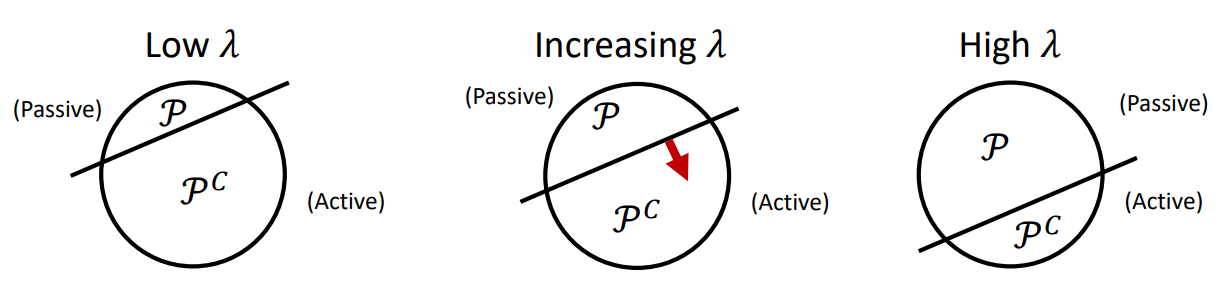
\includegraphics[width=10cm]{images/whittle1.png}
    \caption{}
    \label{fig:whittle1}
\end{figure}


From the above Fig. (\ref{fig:whittle1}) we can see that if an arm $\alpha$ alpha is rested (i.e. in set $\mathcal{P}$) for $\lambda^\alpha$ then it should also be rested for $\lambda_0^\alpha>\lambda^\alpha$ from the above indexability criteria.\\

\begin{definition}
For an arm $\alpha$, Whittle index is defined as the $\lambda^\alpha = \text{inf}\ \{\lambda^\alpha: \alpha \in \mathcal{P}\}$. It is the infimum subsidy $\lambda^\alpha$ one has to pay so that it is equally desirable to give an arm $\alpha$ action and passive action.
\end{definition}
\begin{figure}[htp]
    \centering
    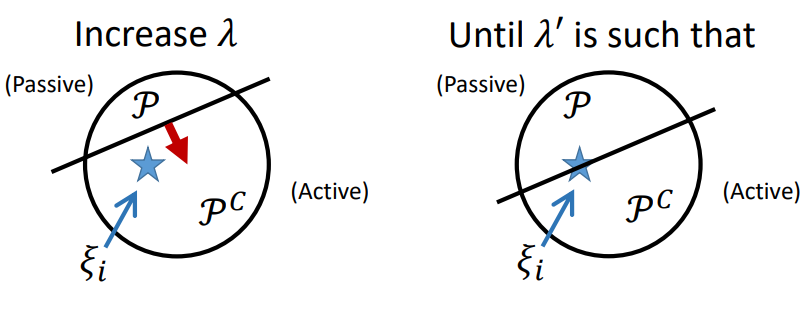
\includegraphics[width=7cm]{images/whittle2.png}
    \caption{Whittle Index $\lambda'$}
    \label{fig:whittle2}
\end{figure}
The above Fig. (\ref{fig:whittle2}) makes the definition more clear, here $\xi_i$ denotes the state and $\lambda'$ is the whittle index.\\

\begin{definition}
A Whittle Index policy is the policy which activates or gives active actions to those $M$ arms out of $N$ which has highest whittle indices $\lambda$.  
\end{definition}
We note that, Whittle Index policy activates arms with highest whittle indices which are those $M$ arms that are last to leave the state set $\mathcal{P}^C$ as the subsidy for the passive action $\lambda$ increases.

\subsection{Q-learning for Whittle Index}
From \cite{avrachenkov2021whittle} the Q-values satisfy the following DP equation
\begin{eqnarray}
Q(i,u) = ur(i,1) + (1-u)(\lambda + r(i,0)) - \rho + \sum_j p(j|i,u)\max_v Q(j,v) \quad \forall i \in \mathcal{S}, u \in \mathcal{A}\ \text{and all $M$ arms}.
\label{Q-DP}
\end{eqnarray}
Where we recall from above that $\rho$ is uniquely specified optimal average reward and $Q$ is unique upto an additive constant.

Whittle index $\lambda(\hat{k})$ is defined as 
\begin{eqnarray}
\lambda(\hat{k}) := r(\hat{k},1) + \sum_jp(j | \hat{k}, 1)V(j)
- r(\hat{k},0)-\sum_jp(j | \hat{k}, 0)V(j). \label{Windex0}
\end{eqnarray}
which is equivalent to solving
\begin{equation}
Q(\hat{k}, 1) - Q(\hat{k}, 0)=0,\quad  \text{for}\  \lambda = \lambda(\hat{k})\label{Windex}
\end{equation}

The proposed Q-learning for Whittle Index takes the following form which is essentially a two time scale optimization algorithm where we update the $Q$-values on a faster time-scale and update the whittle indices $\lambda$ on a faster time scale so that the $Q$-value keep track of the slowly varying $\lambda$. 
\begin{eqnarray}
Q_{n+1}(i,u;\hat{k}) &=& Q_n(i,u;\hat{k})  +  a(\nu(i,u,n)) \times I\{X_n = i, U_n = u\}\Big((1-u)(r(i,0) + \lambda_n(\hat{k})) +  ur(i,1)    \nonumber \\
&& + \ \max_{v\in\mathcal{A}}Q_n(X_{n+1},v;\hat{k})  - f(Q_n{(\hat{k})}) - \ Q_n(i,u;\hat{k})\Big) \label{Q-update0}
\end{eqnarray}
where $\nu(i,u,n)$ is the local clock, $f$ satisfies the Assumption \ref{assmp:lip} and $\lambda_n(\hat{k})$ is the estimated whittle index for state $\hat{k}\in\mathcal{S}$.\\

Whittle index $\lambda(\hat{k})$ for state $\hat{k}$ is updated by the following equation:
\begin{equation}
\lambda_{n+1}(\hat{k}) = \lambda_n(\hat{k}) + b(n) \left( Q_n(\hat{k},1;\hat{k}) - Q_n(\hat{k},0;\hat{k}) \right).
\label{lambda-update}
\end{equation}
where stepsize sequence $\{b(n)\}$ satisfies $\sum_nb(n) = \infty$, $\sum_nb(n)^2 < \infty$ and $b(n) = o(a(n))$.\\
Here we also assume comparable exploration \ref{assmp:exp}.\\

The above method has shown to produce exact whittle indices.\\
We note here that as the state-space grows updating the indices $\lambda$ is inefficient so we update $\lambda$'s for a suitably chosen subset of $\mathcal{S}$ and interpolate.

\subsection{FGDQN for Whittle-Index}
Now, the obvious thing to do when we have a large state $\mathcal{S}$ and action $\mathcal{A}$ space is to use Deep Neural Networks as a function approximators.
We get the following $Q$ iteration for FGDQN by paremeterizing the $Q$ and whittle network with parameters $\theta$ and $\theta'$ respectively.
\begin{eqnarray}
\label{whittleQiteration}
\theta_{n+1} &=& \theta_n - a(n)\Bigg(\overline{(1-U_n)(r(X_n,0) + \lambda_n(\hat{k})) + U_nr(X_n,1)+ \max_{v\in\{0,1\}} Q(X_{n+1}, v; \theta_n,\hat{k}) - f(Q(\hat{k};\theta)) - Q(X_n, U_n;\theta_n,\hat{k})}\times \nonumber \\
&& \left(\nabla_\theta Q(X_{n+1}, v_n; \theta_n,\hat{k})  - \nabla_\theta f(Q(\hat{k};\theta)) - \nabla_\theta Q(X_n, U_n; \theta_n,\hat{k})\right)  + \xi_{n+1}\Bigg)
\end{eqnarray}


Now, we will prove our approach of using Whittle Indices along with FGDQN. Following we derive the iteration for $\theta'$ which is the Whittle Network parameters.\\
As we have seen, whittle index is equivalent to solving for $\lambda(\hat{k}_n)$ the following equation
\begin{equation}
    Q(\hat{k}_n,1) = Q(\hat{k}_n,0)\nonumber
\end{equation}
Substituting $Q(\hat{k}_n,0)$ from the DP Eq. (\ref{Q-DP}) we get
\begin{equation}
    Q(\hat{k}_n,1) = r(\hat{k}_n,0) + \lambda(\hat{k}_n)-\rho+\sum p(\hat{k}_{n+1}|\hat{k}_n,0)\max_{v\in\{0,1\}}Q(\hat{k}_{n+1},v;\theta_n)\nonumber
\end{equation}
which is equivalent to
\begin{equation}
    \lambda(\hat{k}_n) = Q(\hat{k}_n,1)-r(\hat{k}_n,0)+\rho-\sum p(\hat{k}_{n+1}|\hat{k}_n,0)\max_{v\in\{0,1\}}Q(\hat{k}_{n+1},v;\theta_n)\nonumber
\end{equation}  \clearpage
Now, using stochastic approximation we remove the conditional expectation by a real random variable $\xi_{i0}$ with the law $p(\cdot|\hat{k}_n,0)$ and make increment based on our current estimate. We consider a single run $\{X_n=\hat{k}_n,U_n=0\}$ of the controlled Markov chain which gives $\hat{k}_{n+1}$ with the same conditional law. 
\\$\therefore$ We now know have,
\begin{equation}
    \lambda(X_n) = (1-b(n))\lambda(X_n)+ I\{X_n=\hat{k}_n,U_n=0\}b(n)\Big(Q(X_n,1)-r(X_n,0)+\rho-\max_{v\in\{0,1\}}Q(X_{n+1},v;\theta_n)\Big)\nonumber
\end{equation}
We replace $\rho$ with it's current estimate i.e. $f(Q_n)$ to get
\begin{equation}
    \lambda(X_n) = (1-b(n))\lambda(X_n)+ I\{X_n=\hat{k}_n,U_n=0\}b(n)\Big(Q(X_n,1)-r(X_n,0)+f(Q_n)-\max_{v\in\{0,1\}}Q(X_{n+1},v;\theta_n)\Big)\nonumber
\end{equation}
\begin{eqnarray}
\label{whittleiteration}
\lambda(X_n) &=& \lambda(X_n)+ I\{X_n=\hat{k}_n,U_n=0\}b(\mu(i,0,n)) \Big(Q(X_n,1)-r(X_n,0)\nonumber \\&&+f(Q_n)-\max_{v\in\{0,1\}}Q(X_{n+1},v;\theta_n)-\lambda(X_n))\Big)
\end{eqnarray}
here, $\mu(i,0,n)$ is a local clock for Whittle Index and $b=o(n)$ also $a(n)$ and $b(n)$ satisfy the standard Robins-Monro Condition for stochastic approximation.\\

Following we get the iteration for Whittle Index parameters $\theta'$

\begin{eqnarray}
\theta'_{n+1} &=& \theta'_n+b(n)I\{U_n=0\}\times\Big(Q(X_n,1;\theta_n)-r(X_n,0)
\nonumber \\&&+f(Q_n)-\max_{v\in\{0,1\}} Q(X_{n+1}, v; \theta_n)-\lambda(X_n;\theta'_n)\Big)\nabla_{\theta'}\lambda(X_n;\theta'_n)
\label{method2}\end{eqnarray}

So now we have developed Two-Time Scale Optimization Algorithm, wherein we update Q-values according to Eq. (\ref{whittleQiteration}) on a faster time scale and update Whittle Indices for all states using Eq. (\ref{method2}) on a relatively slower time scale.\\
Please refer to Algorithm (\ref{fgdqn_whittle_algorithm}) for the detailed explanation of the implementation.
\clearpage
\section{Experiments}
As a part of experiments I have integrated FGDQN with averaged reward described fully in Algorithm (\ref{fgdqn_algorithm}) in popular PyTorch Reinforcement Learning Libraries.\\
Following are some problems to test our average reward based FGDQN algorithm.
\subsection{Forest Management}
This is a simple MDP problem of Forest Management taken from \cite{avrachenkov2021gradient}. The objective is to maintain an old forest for wildlife and make money by selling the cut wood. 

The state of the forest at time $n$ is $ X_n \in \{0,1,2,3, \cdots, M\}$ where each value of the state represents the age of the forest; $0$ being the youngest and $M$ being the oldest.\\
The forest is managed by two actions: `Wait' and `Cut'. If we apply the action `Cut' at any state, the forest will return to its youngest age, i.e., state $0$. On the other hand, when the action `Wait' is applied, the forest will grow and move to the next state if no fire occurred. Otherwise, with probability $p$, the fire burns the forest after applying the `Wait' action, leaving it at its youngest age (state $0$). \\
Note that if the forest reaches its maximum age, it will remain there unless there is a fire or action `Cut' is performed. Lastly, we only get a reward when the `Cut' action is performed. In this case, the reward is equal to the age of the forest. There is no reward for the action `Wait'.

For $p=0.05$ and $M=10$, the optimal policy obtained from policy iteration algorithm is [0, 1, 1, 1, 1, 1, 1, 1, 1, 1].\\
I have experimented for two variants of the reference value function $f$, one for fixed state-action pair of age 0 and action `Wait' and other one is using average of all Q-values as shown in Fig. (\ref{Forest Management}). \\
The Optimal policies obtained are:\\
Variant 1 : [0, 1, 1, 1, 1, 1, 1, 1, 1, 1]\\
Variant 2 : [0, 0, 1, 1, 1, 1, 1, 1, 1, 1] (1-bit error).
\begin{figure}[H]
     \captionsetup[subfigure]{justification=centering}
     \centering
     %\hspace{-0.26\linewidth}
     \begin{subfigure}{0.48\linewidth}
         \centering
         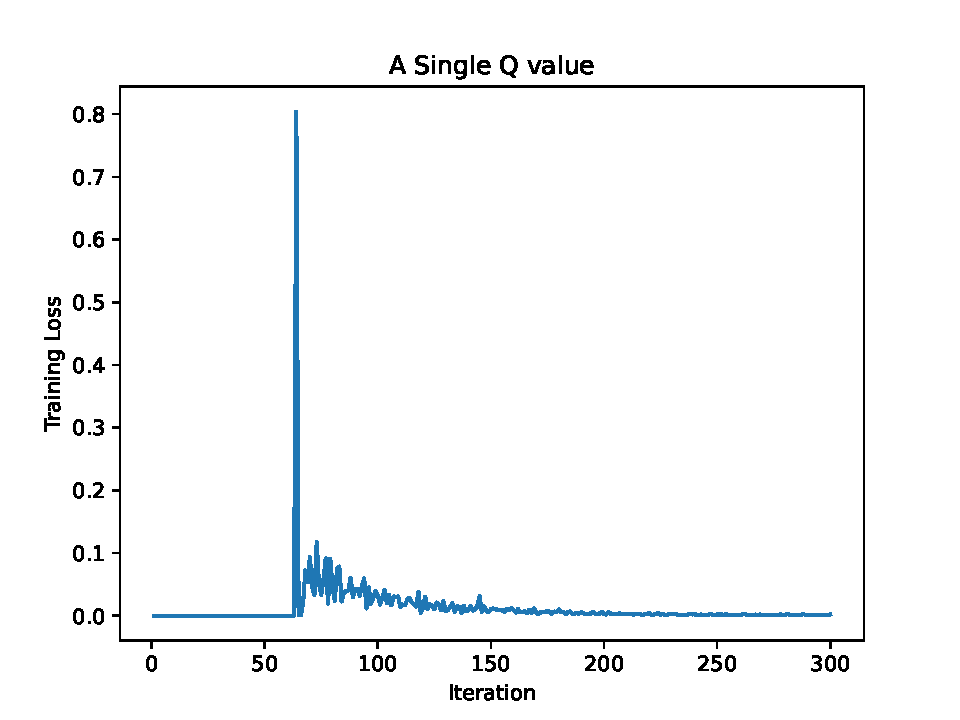
\includegraphics[width=1\linewidth]{variant1.pdf}
         \caption*{$f(Q) = Q(X_0,U_0)$}
         \label{}
     \end{subfigure}
     %\hspace{0.2\linewidth}
     \begin{subfigure}{0.48\linewidth}
         \centering
         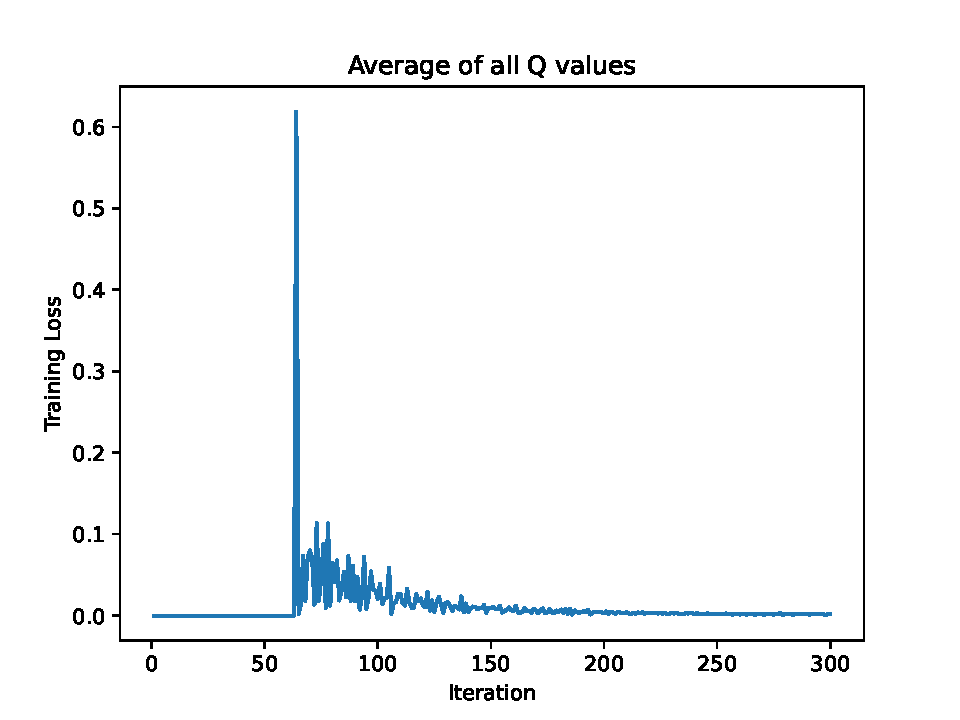
\includegraphics[width=1\linewidth]{variant2.pdf}
         \caption*{$f(Q) = \overline{Q(X_0,U_0)}$}
         \label{}
     \end{subfigure}
     %\hspace{0.2\linewidth}
     %\hspace{0.2\linewidth}
     \caption{Forest Management}
     \label{Forest Management}
\end{figure}


\subsection{Catcher}
This is a game environment from \cite{tasfi2016PLE} in which the aim of the agent is to catch the falling fruit with it's paddle.\\
Reward is +1 for successful fruit catch and -1 if the fruit is not caught.\\
The player is allowed to take only two actions of either moving right or left.\\
The states are non-visual representation of the game such as player's x position and velocity, fruits x and y position.
Following are the results, the agent learnt to catch the fruits pretty well but it hasn't mastered it very well. I hope to train it more longer in the hope of getting good results.
\begin{figure}[htbp]
    \centering
    \includesvg[width=10cm]{images/catcher/eval_mean_reward.svg}
    \caption{Reward}
    \label{fig:my_label}
\end{figure}
    
\begin{figure}[htbp]
    \centering
    \includesvg[width=10cm]{images/catcher/train_loss.svg}
    \caption{Training Loss}
    \label{fig:my_label}
\end{figure}

\subsection{Whittle Indices}

\subsubsection{Circulant Dynamics}
We consider a simple RMAB problem of Circulant Dynamics from  \cite{circulantdynamics}, where we have $I$ projects out of which we can do only $K$ at a particular instant on priority basis. Each project has a underlying Markov chain for both Active $(u=1)$ and Passive action $(u=0)$. These two problems are taken from \cite{avrachenkov2021whittle} as they serve as a basis for most of the other types of RMAB problems.

\begin{figure}[H]
     \captionsetup[subfigure]{justification=centering}
     \centering
     %\hspace{-0.26\linewidth}
     \begin{subfigure}{0.2\linewidth}
         \centering
         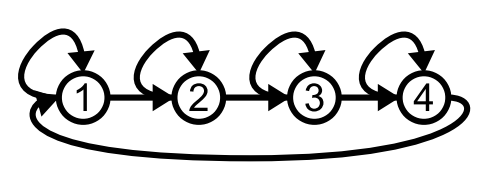
\includegraphics[width=0.7\linewidth]{images/circac.png}
         \caption{Action Action}
         \label{}
     \end{subfigure}
     \begin{subfigure}{0.2\linewidth}
         \centering
         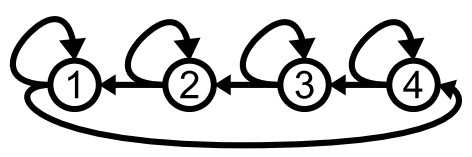
\includegraphics[width=0.7\linewidth]{images/circpas.png}
         \caption{Passive Action}
         \label{}
     \end{subfigure}
     %\hspace{0.2\linewidth}
     %\hspace{0.2\linewidth}
     \caption{Underlying Markov chains of the Circulant Dynamics Problem}
     \label{Circulant Dynamics}
\end{figure}
Consider the transition probability matrix $P_0=\left[\begin{array}{cccc}
{\small 1/2} & 0 & 0 & 1/2\\
1/2 & 1/2 & 0 & 0\\
0 & 1/2 & 1/2 & 0\\
0 & 0 & 1/2 & 1/2
\end{array}\right], \quad \mbox{and} \quad
P_1=P_0^T,$ for passive and active action respectively. \\The rewards here do not depend on action and are given by $R(1,0)=R(1,1)=-1$, $R(2,0)=R(2,1)=0$, $R(3,0)=R(3,1)=0$, and $R(4,0)=R(4,1)=1$. Where $R(s,u)$ denotes the reward in state $s$ after taking action $u$.
Intuitively, there is a preference to activate an arm when the arm is in
state 3.\\
For experimentation, we consider a scenario with $N=100$ arms, out of which $M=20$ are active
at each time. The exact whittle indices for this problem turns out to be $\lambda(1)=-1/2$, $\lambda(2)=1/2$, $\lambda(3)=1$, and $\lambda(4)=-1$, which
give priority to state 3.\\
Here, we make two Neural Networks one for $\lambda$ and the other for $Q$ with parameters $\theta'$ and $\theta$ respectively. Please refer to \ref{fgdqn_whittle_algorithm} for more detailed explanation of the algorithm.\\
This problem is very stochastic in nature as at a particular state there is $1/2$ probability for both actions to move to the other respective states. The order of the Whittle Indices settles pretty quickly as shown in Fig. \ref{Whittle Indices1}, but the order of the exact indices doesn't seem to match here. As it is clear the results show $\lambda(2)>\lambda(3)$ which should be the other way around. One thing to note here, that the $Q$-loss was pretty high even after $10000$ iteration, more hyperparameter tuning will surely give better results.
\begin{figure}[H]
\ContinuedFloat
     \captionsetup[subfigure]{justification=centering}
     \centering
     %\hspace{-0.26\linewidth}
     \begin{subfigure}{0.48\linewidth}
         \centering
         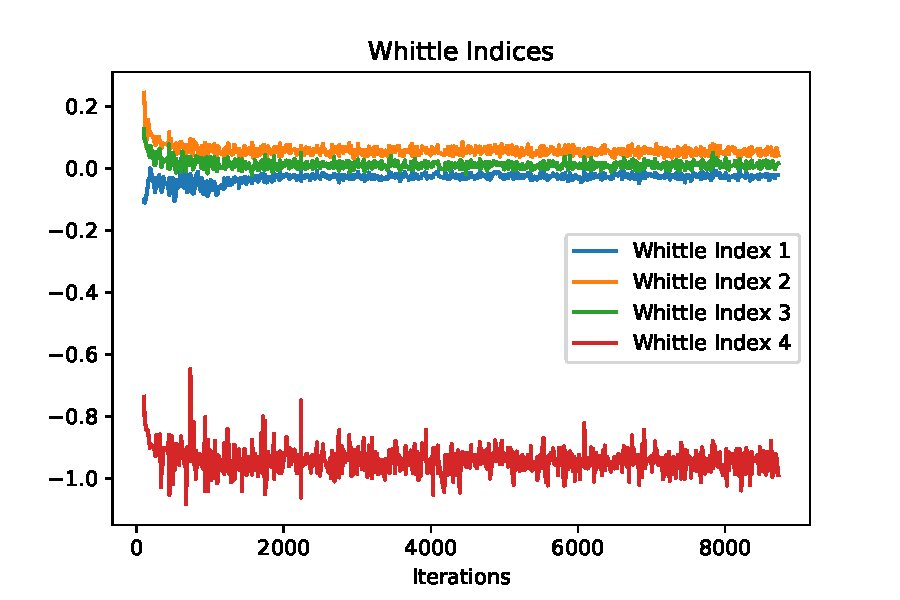
\includegraphics[width=1\linewidth]{images/whittle1/all.pdf}
         \caption{Whittle Indices}
         \label{Whittle Indices1}
     \end{subfigure}
     \begin{subfigure}{0.48\linewidth}
         \centering
         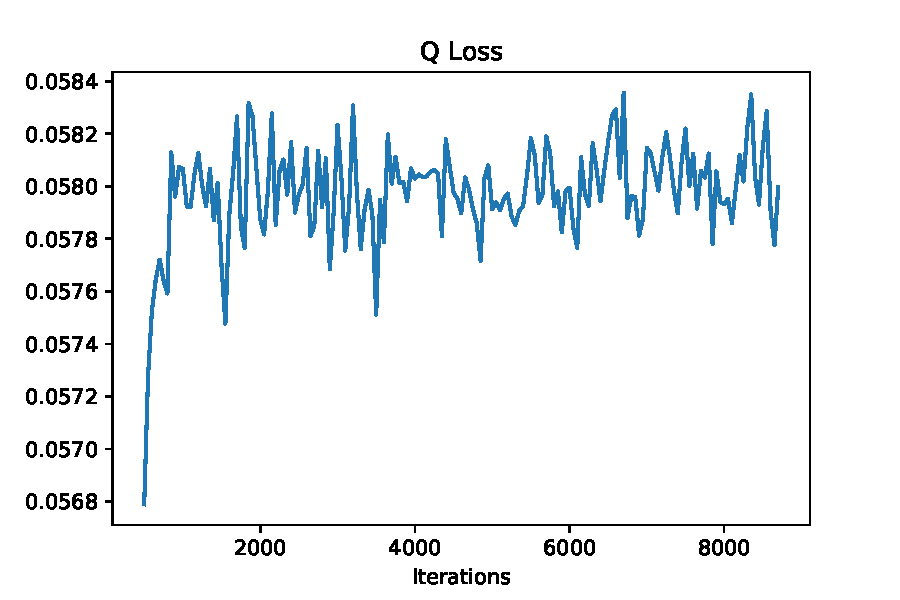
\includegraphics[width=1\linewidth]{images/whittle1/Q Loss.pdf}
         \caption{Q loss}
         \label{}
     \end{subfigure}
     
     \begin{subfigure}{0.48\linewidth}
         \centering
         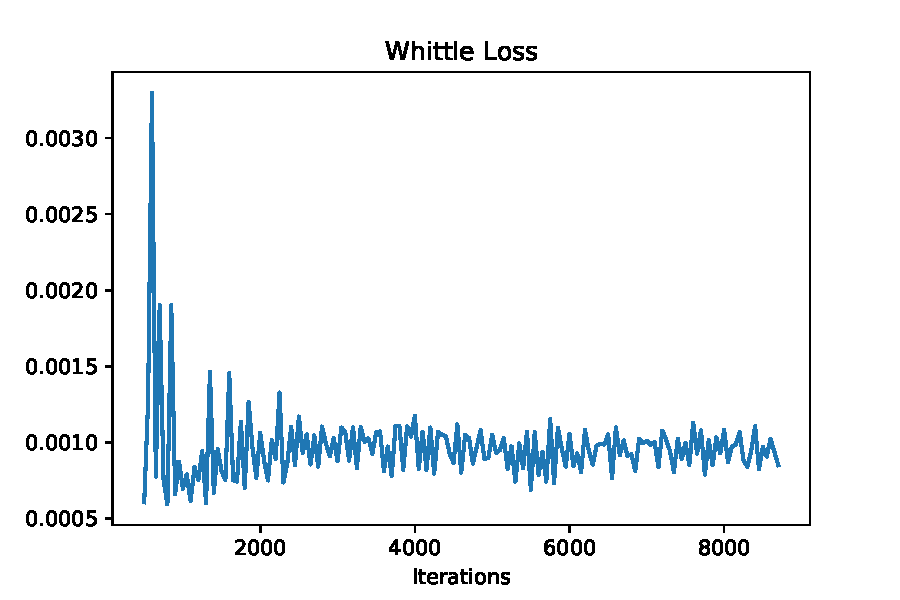
\includegraphics[width=1\linewidth]{images/whittle1/Whittle Loss.pdf}
         \caption{Whittle loss}
         \label{}
     \end{subfigure}
     %\hspace{0.2\linewidth}
     %\hspace{0.2\linewidth}
     \caption{Circulant Dynamics}
     \label{}
\end{figure}
\subsubsection{Circulant Dynamics with Restart}
Now we consider an example where the active action forces an arm
to restart from some state. We consider an example with 5 states,
where in the passive mode ($u=0$) an arm has tendency to go up the state space, i.e.,
$$
P_0=\left[\begin{array}{ccccc}
1/10 & 9/10 & 0 & 0 & 0\\
1/10 & 0 & 9/10 & 0 & 0\\
1/10 & 0 & 0 & 9/10 & 0\\
1/10 & 0 & 0 & 0 & 9/10\\
1/10 & 0 & 0 & 0 & 9/10
\end{array}\right],
$$
whereas in the active mode ($u=1$) the arm restarts from state 1 with probability 1, i.e.,
$$
P_1=\left[\begin{array}{ccccc}
1 & 0 & 0 & 0 & 0\\
1 & 0 & 0 & 0 & 0\\
1 & 0 & 0 & 0 & 0\\
1 & 0 & 0 & 0 & 0\\
1 & 0 & 0 & 0 & 0
\end{array}\right].
$$
The rewards in the passive mode are given by $R(k,0)=\alpha^k$ ($\alpha$ is taken to be 0.9) and the rewards in the active mode are all zero.\\
We again take $N=100$ and $M=20$ for experimentation. \\
The results here are very good, as we can see in Fig. (\ref{Whittle Indices 2}) the order of the indices settles pretty quickly and both the $Q$ and Whittle loss approaches $0$ in about $500$ iterations.

\begin{figure}[H]
     \captionsetup[subfigure]{justification=centering}
     \centering
     %\hspace{-0.26\linewidth}
     \begin{subfigure}{0.48\linewidth}
         \centering
         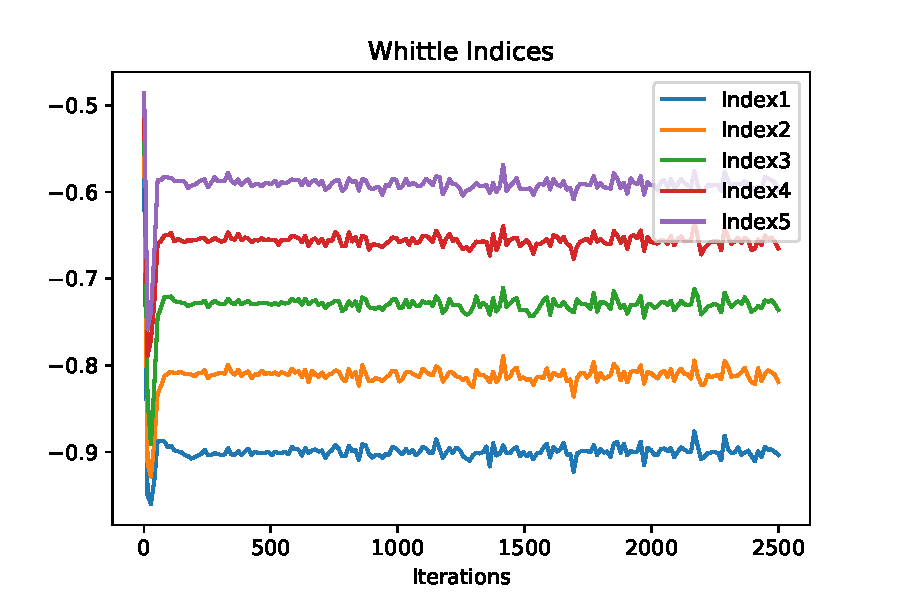
\includegraphics[width=1\linewidth]{images/whittle2/Indices.pdf}
         \caption{Whittle Indices}
         \label{Whittle Indices 2}
     \end{subfigure}
     \begin{subfigure}{0.48\linewidth}
         \centering
         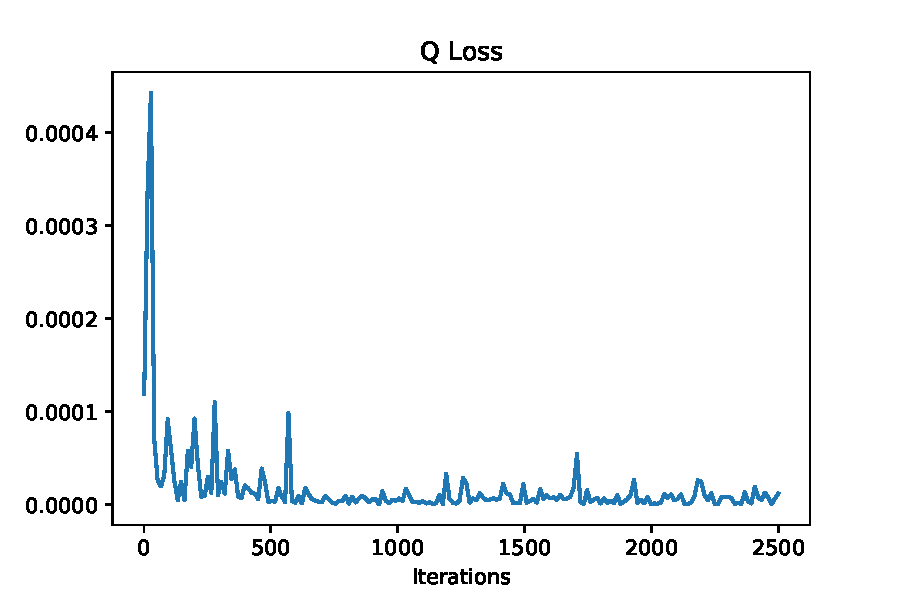
\includegraphics[width=1\linewidth]{images/whittle2/Q Loss.pdf}
         \caption{Q loss}
         \label{}
     \end{subfigure}
     %\hspace{0.2\linewidth}
     %\hspace{0.2\linewidth}
     \caption{Circulant Dynamics with Restart}
\end{figure}
\subsection{More Experiments}
Apart from this, I have experimented on some games like Catch, Tic-Tac-Toe, Deep Sea from OpenSpiel \cite{openspiel}, these games are specifically made to test various aspect of an algorithm. I further tested on a Toy Autonomous Driving Environment \cite{highway-env}, for problems like Intersection, Racetrack. I want to give a shoutout to the amazing library Stable-Baselines3 \cite{stable-baselines3} which made my implementation easier and faster. I refer reader to go through the codebase and supplementary materials to find more about their implementation and to try the code yourselves.

\section{Acknowledgments}
I want to sincerely thank Prof. Vivek Borkar for his guidance throughout the course of this project work. He is one of the patient and dedicated Professors I have ever met. His dedication toward research motivates me alot. I also want to thank Dr. Kishor Patil for his valuable discussion and Dr. Konstantin Avrachenkov for his valuable insights.\\
Lastly, I'm very grateful to my parents, my sister and friends and I consider myself very lucky to have them. 
\section{Appendix}
\begin{algorithm}[H]\label{algo1}
\SetKwInOut{Input}{Input}
\SetKwInOut{Output}{Output}
\SetAlgoLined
% \KwResult{Write here the result }
 \textbf{Input:} replay memory $\mathcal{D}$ of size $M$, minibatch size $B$, number of episodes $N$, maximal
length of an episode $T$, exploration probability $\epsilon$.\\
 Initialise the weights $\theta$ randomly for the Q-Network.\\
Receive initial observation $s_1$.\\
%Update $\psi$ from parameters $\psi^+$ of the parameter server.\\
\For{Episode = 1 to N}{
\For{n = $1$ to $T$}{
\eIf{Uni[0,1] $<$ $\epsilon$ }{Select action $U_n$ at random.}
{
$U_n = Argmax_{u} Q(X_n,u;\theta)$
}
Execute the action and take a step in the RL environment.\\
Observe the reward $R_n$ and obtain next state $X_{n+1}$.\\
Store the tuple $(X_n, U_n, R_n, X_{n+1})$ in $\mathcal{D}$.\\
Sample random minibatch of $B$ tuples from $\mathcal{D}$.
\For{ k =  $1$ to $B$}{
Sample all tuples $(X_j, U_j, R_j, X_{j+1})$ with a fix state-action pair $(X_j = X_k, U_j = U_k)$ from $\mathcal{D}$
\[Set\, Z_j = \begin{cases} R_j, & \mbox{for terminal state,} \\
R_j + \max_{u} Q(X_{j+1},u;\theta) - Q(x_0, y_0;\theta) & \mbox{otherwise.}\end{cases}\]\\
Compute gradients and using Eq. (\ref{eqn:fgdqnavg})
update parameters $\theta$.\\
}
}}

\caption{Full Gradient DQN (FG-DQN) for Average Reward} 
\label{fgdqn_algorithm}
\end{algorithm}
\clearpage
\begin{algorithm}[H]\label{algo2}
\SetKwInOut{Input}{Input}
\SetKwInOut{Output}{Output}
\SetAlgoLined
% \KwResult{Write here the result }
 \textbf{Input:} replay memory $\mathcal{D}$ of size $M$, minibatch size $B$ for Q iteration and $C$ for $\lambda$ iteration, number of episodes $N$, maximal length of an episode $T$, discount factor $\gamma$, exploration probability $\epsilon$, whittle index $\lambda$.\\
 Initialise the weights $\theta \ \& \ \theta'$ randomly for the Q-Network and Whittle-Network.\\
 Consider RMABP with $I$ projects such that at every time step $K$ of them are active. \\
Denote state of the system at time $n$ as $S(n) = (s_1(n),\cdots,s_i(n),\cdots,s_I(n))$ where $s_i(n)$ is a state of project $i\in\{1,2,\cdots,I\}$ 
 \\
\For{n = $1$ to $T$}{
  \For{s = $1$ to $d$}{ 
  %Update $\psi$ from parameters $\psi^+$ of the parameter server.\\
  \vspace{\baselineskip}
  Select actions $U(n) = (u_1(n),\cdots,u_i(n),\cdots,u_I(n)))$ at random such that $\sum_{i=1}^{I}u_i(n)=K$.
  \vspace{\baselineskip}\\
  Execute actions and take a step.\\
  Observe the rewards $R(n) = (r_1(n),\cdots,r_I(n))$ and obtain next state of the system $S(n+1)$.\\
  Store all the tuples $(S(n),U(n),R(n),S(n+1))$ in $\mathcal{D}$.\\
  \vspace{\baselineskip}
  Sample random minibatch of $B$ tuples from $\mathcal{D}$.\\
  \For{ $a =  \{0,1\}$}{
    Sample all tuples $(X_j, U_j, R_j, X_{j+1})$ of size $B$ with a fix state-action pair $(X_j = s, U_j = a)$ from $\mathcal{D}$\\
    \For{$\hat{k}$ = $1$ to $d$}{\[Set\, Z_j = (1-U_j)(R_j+\lambda(\hat{k}))+U_jR_j + \max_{v} Q(X_{j+1},v;\theta,\hat{k}) - f(Q(\hat{k};\theta)) \]
    \\
    Compute gradients and using Eq. (\ref{whittleQiteration}) update parameters $\theta$.\\}\\
  }}
  \vspace{\baselineskip}\\
  On slower time-scale \textbf{do}\\
  Sample all tuples $(X_k, U_k, R_k, X_{k+1})$ of size $B$ with fix action $U_k = 0$ from $\mathcal{D}${\[Set\, Z_k = Q(X_k,1;\theta_n)-r(X_k,0)+f(Q(X_n,\theta_n))
-\max_{v\in\{0,1\}} Q(X_{k+1}, v; \theta_n)\]
Compute gradients and using Eq. (\ref{method2}) update parameters $\theta'$.}
 }
\caption{Whittle Indices with FGDQN}
\label{fgdqn_whittle_algorithm}
\end{algorithm}

% where $v_n = \underset{{v\in\{0,1\}}}{\max}{Q(X_{n+1}}, v; \theta_n,\hat{k})$
% \[S = \{1, 2,..., d\} \hspace{60pt} f(Q(X_n)) = \dfrac{1}{2d}\sum_{i\in S}(Q(i,0)+Q(i,1))\]
% Thus for each $\hat{k} \in S$, we perform the iteration
% \begin{eqnarray}
% Q_{n+1}(i,u;\hat{k}) = Q_n(i,u;\hat{k})  +  a(\nu(i,u,n)) \times I\{X_n = i, U_n = u\}\Big((1-u)(r(i,0) + \lambda_n(\hat{k})) +  ur(i,1) + \max_{v\in\U}Q_n(X_{n+1},v;\hat{k})  \nonumber \\- f(Q_n{(\hat{k})}) - \ Q_n(i,u;\hat{k})\Big) \nonumber
% \end{eqnarray}

% along with an update for learning the Whittle index $\lambda(\hat{k})$ for state $\hat{k}$ given by:
% with a prescribed stepsize sequence $\{b(n)\}$ satisfying $\sum_nb(n) = \infty$, $\sum_nb(n)^2 < \infty$ and $b(n) = o(a(n))$, do
% \begin{equation}
% \lambda_{n+1}(\hat{k}) = \lambda_n(\hat{k}) + b(n) \left( Q_n(\hat{k},1;\hat{k}) - Q_n(\hat{k},0;\hat{k}) \right).
% \label{lambda-update}
% \end{equation}
% We use the `hat notation' $\hat{k}$ to emphasize that $\hat{k}$ is the $\hat{k}$-th component of the Whittle index
% estimation evolving on the slow time scale.

% We need to estimate $Q(i,u;\hat{k})$ for each arm $\alpha$.\\
% In the case of homogeneous arms and shared memory architecture, we need to update only
% $2d^2+d$ variables, whereas they would have been $(2d)^N$ with Q-learning applied directly without the Whittle scheme.\\

% We assume Whittle index $\lambda$ to be of the form
% \[\lambda(i,z)=\sum_kz_kf_k(i),i\in S\]
% where $f:S\mapsto \mathcal{R}$ are prescribed basis functions and we learn the parameter vector $z_k = [z_1,\cdots,z_s]$ as follows
% \begin{eqnarray}
% z_{n+1} = z_n+b(n)I\{U_n=0\}\times\Big(Q(X_n,1;\theta_n)-r(X_n,0)
% -\max_{v\in\{0,1\}} Q(X_{n+1}, v; \theta_n)-\lambda(X_n;z_n)\Big)\nabla_z\lambda(X_n;\theta_n)
% \label{z iteration}\end{eqnarray}
% \clearpage
% \begin{eqnarray}
% Q_{n+1}(i,u;\hat{k}) = Q_n(i,u;\hat{k})  +  a(\nu(i,u,n)) \times I\{X_n = i, U_n = u\}\Big((1-u)(r(i,0) + \lambda_n(\hat{k})) +  ur(i,1) \ \max_{v\in\U}Q_n(X_{n+1},v;\hat{k})  \nonumber \\- f(Q_n{(\hat{k})}) - \ Q_n(i,u;\hat{k})\Big) \nonumber
% \end{eqnarray}

\clearpage
\subsection{Implementation Details}
The below snippet shows how the $mse\_loss$ of PyTorch \cite{pytorch} works which allowed us to implement our algorithms in a very elegant way.\\
Following are the equations corresponding to $loss.backward()$ in Pytorch.
\begin{align*}
    mse\_loss(pred,target)\\
    loss = (pred-target)^2\\
    \nabla_{\theta} loss = 2(pred-target)(\nabla_{\theta}pred-\nabla_{\theta}target) \\
    \theta_{n} \leftarrow \theta_{n-1} - \gamma \nabla_{\theta} f(\theta_{n-1})\\
    \theta_{n} \leftarrow \theta_{n-1} - \gamma 2(pred-target)(\nabla_{\theta}pred-\nabla_{\theta}target)\\
    \theta_{n} \leftarrow \theta_{n-1} - \gamma 2(target-pred)(\nabla_{\theta}target-\nabla_{\theta}pred)\\
    \theta_{n} \leftarrow \theta_{n-1} + \gamma 2(target-pred)(\nabla_{\theta}pred-\nabla_{\theta}target)
    % mse\_loss(target,out)
    % \\
    % loss = (target-out)^2\\
    % \theta \leftarrow \theta - \eta(\text{target}- \text{out})(\nabla_\theta \text{target}- \nabla_\theta  \text{out})
\end{align*}

Details:
\begin{eqnarray}
\label{eqn:pytorchfgdn}
\theta_{n} \leftarrow \theta_{n-1} - \gamma 2(target-pred)(\nabla_{\theta}target-\nabla_{\theta}pred)
\end{eqnarray}

\begin{eqnarray}
\label{eqn:originalfgdqn}
\theta_{n+1} &=& \theta_n - a(n)\left(r(X_n,U_n) +\max_v Q(X_{n+1}, v; \theta_n) -f(Q;\theta_n) - Q(X_n, U_n;\theta_n)\right)\times \nonumber \\
&& \Big(\nabla_\theta Q(X_{n+1}, v_n; \theta_n) - \nabla_\theta f(Q;\theta_n) - \nabla_\theta Q(X_n, U_n; \theta_n)\Big) 
\end{eqnarray}
where $v_n \in \text{argmax} Q(X_{n+1},\cdot,\theta_n)$

Above  two equations Eq. (\ref{eqn:pytorchfgdn}) \& Eq. (\ref{eqn:originalfgdqn}) resembles, where\\
$target$ is the average reward Q target and $pred$ is predicted Q value from the Q network.
\begin{align*}
    target &= r(X_n,U_n) +\max_v Q(X_{n+1}, v; \theta_n) -f(Q;\theta_n) \\
    pred &= Q(X_n, U_n;\theta_n)
\end{align*}
    
\clearpage    
\subsubsection{New Implementation}
For simplicity assume the fixed state action pair as $(X,U)$. \\
Now, from the replay buffer sample all the transitions with this fixed state action pair as $(X,U)$. Let's say we get $(X,U,R_1,X'_1), (X,U,R_2,X'_2)$ and $(X,U,R_3,X'_3)$ and hence we have a batch size $B$ of 3.

Let's denote 
\begin{align*}
    target_n &= R_n +\max_v Q(X'_n, v; \theta_n) -f(Q;\theta) \\
    pred_n &= Q(X, U;\theta)
\end{align*}
Now, we compute $diff = \dfrac{(target_1-pred_1)+(target_2-pred_2)+(target_3-pred_3)}{3}$ \\using $torch.mean(target\_batch-pred\_batch)$.\\
This is essentially our term under the bar in the FGDQN equation.\\

Now we compute it's gradient to get,\\
$\nabla_\theta diff = \dfrac{(\nabla_\theta target_1-\nabla_\theta pred_1)+(\nabla_\theta target_2-\nabla_\theta pred_2)+(\nabla_\theta target_3-\nabla_\theta pred_3)}{3}$.\\

Now calculate $diff \times \nabla_\theta diff$, to get\\ 
$final\_grad = \dfrac{diff \times (\nabla_\theta target_1-\nabla_\theta pred_1)+diff \times (\nabla_\theta target_2-\nabla_\theta pred_2)+diff \times (\nabla_\theta target_3-\nabla_\theta pred_3)}{3}$.\\

$final\_grad$ is essentially the term we wanted for the FGDQN iteration. 
Now we simply do, 

\begin{align*}
\theta' \leftarrow \theta - \gamma(final\_grad)
\end{align*}


\subsubsection{Mistake in previous Implementation}
In my previous implementation I simply calculated the gradient of \\

$loss = \dfrac{(target_1-pred_1)^2+(target_2-pred_2)^2+(target_3-pred_3)^2}{3}$
which is 

$\nabla_\theta loss = \dfrac{2(target_1-pred_1)(\nabla_\theta target_1-\nabla_\theta pred_1)+2(target_2-pred_2)(\nabla_\theta target_2-\nabla_\theta pred_2)+\cdots}{3}$

and then did

\begin{align*}
\theta' \leftarrow \theta - \gamma(\nabla_\theta loss)
\end{align*}
    
This doesn't resemble the FGDQN iteration, since here we are not multiplying the average (the term with the overline in iteration) with each gradient.
    
    
    
    
    
    
    
    
\clearpage
Consider parametrized families $\lambda(k,\sigma)$ and $Q(i , u; \theta, \sigma)$ where we render explicit the implicit dependence of $Q$ on $\lambda$ and therefore $\sigma$. Consider
\begin{eqnarray*}
\lefteqn{\theta_{n+1} \ = \  \theta_n \ - \  a(n)\Big(\nabla_\theta Q(X_{n+1},v_n;\theta_n,\sigma_n) \ - \ \nabla_\theta f(Q(\theta,\sigma_n))\Big|_{\theta = \theta_n} }\\
&& - \ \nabla_\theta Q(X_n,U_n;\theta_n,\sigma_n) \ \Big)\times  \\
&&\overline{\Big((1-U_n)(r(X_n,0) + \lambda(X_n,\sigma_n)) + U_nr_n(X_n,1) + \max_{v\in\{0,1\}}Q(X_{n+1},v;\theta_n,\sigma_n)}\\
&&\overline{ - \ f(Q(\theta_n,\sigma_n)) - Q(X_n,U_n;\theta_n,\sigma_n)\Big)} + a(n) \xi_{n+1},\\
\lefteqn{\sigma_{n+1} = \sigma_n - b(n)\overline{\Big(Q(X_n, 1;\theta_n,\sigma_n) - r(X_n,0)  + \ f(Q(X_n,0;\theta_n,\sigma_n))}}\\
&& \overline{- \max_{v\in\{0,1\}}Q(X_{n+1},v;\theta_n,\sigma_n) - \lambda(X_n,\sigma_n)\Big)} \times \\
&& \Big(\nabla_\sigma Q(X_{n+1},v_n;\theta_n,\sigma_n) \ - \ \nabla_\sigma f(Q(\theta_n,\sigma))\Big|_{\sigma = \sigma_n} \\
&& - \ \nabla_\sigma Q(X_n,U_n;\theta_n,\sigma_n) - \nabla_\sigma\lambda(X_n,\sigma_n)\Big)
\end{eqnarray*}
The $\theta_n$ iteration is the SGD for the mean square error
\begin{eqnarray*}
\lefteqn{\mathcal{E}_1 := E\Big[\Big\|(1-U_n)(r(X_n,0) + \lambda(X_n,\sigma_n)) + U_nr_n(X_n,1) }\\
&&+ \ \max_{v\in\{0,1\}}Q(X_{n+1},v;\theta_n,\sigma_n)
 - \ f(Q(\theta_n,\sigma_n)) - Q(X_n,U_n;\theta_n,\sigma_n)\Big\|^2\Big].
\end{eqnarray*}
The $\sigma_n$ iteration is the SGD to minimize the mean square error
\begin{eqnarray*}
\lefteqn{\mathcal{E}_2 := E\Big[\Big\|Q(X_n, 1;\theta_n,\sigma_n) - r(X_n,0)  + \ f(Q(X_n,0;\theta_n,\sigma_n))}\\
&& - \max_{v\in\{0,1\}}Q(X_{n+1},v;\theta_n,\sigma_n) - \lambda(X_n,\sigma_n)\Big\|^2\Big].
\end{eqnarray*}
\clearpage

Consider parametrized families $\lambda(k,\sigma)$ and $Q(i , u, \lambda; \theta)$ where we render the implicit dependence of $Q$ on $\lambda$ by taking it as a input to the Q-network.

\begin{eqnarray*}
\lefteqn{\theta_{n+1} \ = \  \theta_n \ - \  a(n)\Big(\nabla_\theta Q(X_{n+1},v_n,\lambda(X_{n+1};\sigma_n);\theta_n)\ - \ \nabla_\sigma f(Q(X_n,U_n,\lambda(X_n;\sigma_n);\theta_n))}\nonumber\\
&& - \ \nabla_\theta Q(X_n,U_n,\lambda(X_n;\sigma_n);\theta_n)\ \Big)\times  \nonumber\\
&&\overline{\Big((1-U_n)(r(X_n,0) + \lambda(X_n;\sigma_n)) + U_nr_n(X_n,1) + \max_{v\in\{0,1\}}Q(X_{n+1},v,\lambda(X_{n+1};\sigma_n);\theta_n)}\nonumber\\
&&\overline{ - \ f(Q(X_n,U_n,\lambda(X_n;\sigma_n);\theta_n))
 - Q(X_n,U_n,\lambda(X_n;\sigma_n);\theta_n)\Big)} + a(n) \xi_{n+1},\\\nonumber\\
\lefteqn{\sigma_{n+1} = \sigma_n - b(n)\overline{\Big(Q(X_n, 1,\lambda(X_n;\sigma_n);\theta_n) - r(X_n,0)  + \ f(Q(X_n,0,\lambda(X_n;\sigma_n);\theta_n))}}\nonumber\\
&& \overline{- \max_{v\in\{0,1\}}Q(X_{n+1},v,\lambda(X_{n+1};\sigma_n);\theta_n) - \lambda(X_n;\sigma_n)\Big)} \times \nonumber\\
&& \Big(\nabla_\sigma Q(X_n,U_n,\lambda(X_n;\sigma_n);\theta_n)  \ + \ \nabla_\sigma f(Q(X_n,0,\lambda(X_n;\sigma_n);\theta_n)) \nonumber\\
&& - \ \nabla_\sigma Q(X_{n+1},v_n,\lambda(X_n;\sigma_n);\theta_n) - \nabla_\sigma\lambda(X_n;\sigma_n)\Big)\\
\end{eqnarray*}





\clearpage
% \begin{thebibliography}{1}
% \newcommand{\enquote}[1]{``#1''}
% \bibitem{markov}
% {Robert G. Gallager, Finite-State Markov Chains, MIT OCW}
% \bibitem{vol1}
% {Dynamic Programming and Optimal Control (Dimitri P. Bertsekas), Athena Scientific, volume I, 2005.
% }
% \bibitem{vol2}{Bertsekas, D. P. (2012). Dynamic Programming and Optimal Control, Vol. II. Athena Scientific, 4th
% edition}
% \end{thebibliography}
\bibliographystyle{plain}
\bibliography{references.bib}
\end{document}
